\chapter{نتایج و ارزیابی}
\section{مقدمه}
سیستم تشخیص حرکات دست نقش مهمی در زمینه ایجاد تعامل کارآمد بین انسان و ماشین ایفا می‌کند. پیاده‌سازی این سیستم با استفاده از تشخیص علائم دست، باعث افزایش وسیعی در استفاده کاربردی از هوش مصنوعی  در صنعت فناوری می‌شود. در این پروژه، 
معماری‌های گوناگونی مانند شبکه‌های عصبی پیچشی، شبکه‌های حافظه کوتاه‌مدت بلند، و شبکه‌های عصبی چندلایه‌ای پرسپترونی مورد آزمایش قرار گرفتند تا بهترین پیاده‌سازی برای تشخیص حرکات دست انتخاب شود. 
\\
در این فصل، به بررسی نتایج به‌دست‌آمده از این پیاده‌سازی‌های متفاوت می‌پردازیم و دقت و عملکرد سیستم در شرایط مختلف را ارزیابی می‌کنیم. همچنین، نقاط قوت و ضعف هر یک از معماری‌های مورد استفاده 
را تحلیل کرده و پیشنهاداتی برای بهبود سیستم ارائه می‌دهیم. هدف این فصل، ارائه یک تحلیل جامع از کارایی سیستم و شناخت دقیق‌تر از عواملی است که می‌توانند به ارتقاء عملکرد آن کمک کنند.


\section{ارزیابی عملکرد مدل‌ها}

این پروژه با مدل‌های گوناگونی پیاده‌سازی شده است تا بتوان بهترین آنها را برای نتیجه نهایی بر روی پهپاد اجرا کرد. معیارهای ارزیابی شامل دقت، صحت \LTRfootnote{Precision}، فراخوانی\LTRfootnote{Recall}، امتیاز \lr{F1} و
تعداد نمونه‌ها برای هر یک از علائم‌ها می‌باشد.
\\
معیار‌های دقت، صحت، فراخوانی و امتیاز \lr{F1} معیارهای ضروری برای ارزیابی عملکرد مدل‌های بینایی ماشین و یادگیری عمیق هستند. این معیار‌ها هر دو نتیجه مثبت کاذب و منفی کاذب را در نظر
می‌گیرند و درک دقیقی از قابلیت‌های پیش بینی یک مدل را ارائه می‌دهند. این ارزیابی دقیق با برجسته کردن نقاط قوت و ضعف خاص هر مدل, به اصلاح مدل کمک می‌کند.
\subsection{دقت}
دقت مدل معیاری است که نشان می‌دهد یک مدل یادگیری عمیق تا چه اندازه قادر به پیش‌بینی یا تصمیم‌گیری صحیح بر اساس داده‌ها است. این معیار به صورت نسبت مجموع مثبت و منفی واقعی به تعداد کل نمونه‌ها محاسبه می‌شود.
\\
دقت، بصری‌ترین معیار عملکرد است و به نسبت مشاهدات پیش‌بینی شده صحیح به کل مشاهدات اشاره دارد. این معیار برای مقایسه عملکرد مدل‌های مختلف و ارزیابی اثربخشی یک مدل خاص برای یک وظیفه معین استفاده می‌شود. دقت زمانی مناسب است که توزیع کلاس‌ها متعادل باشد و هزینه‌ نتیجه‌های مثبت کاذب و منفی کاذب مشابه باشند \cite{Accuracy53:online}.
\begin{equation}
    Accuracy = \frac{True \, Positives + True \, Negatives}{True \, Positives + True \, Negatives + False \, Positives + False \, Negatives}
\end{equation}


\begin{table}[h!]
    \centering
    \begin{tabular}{||c c c c||}
     \hline
     \rule{0pt}{3ex} معماری مدل & دوره & دقت داده آموزش & دقت داده تست  \\ [1.5ex]
     \hline
     \hline
     \rule{0pt}{0.5ex} & & & \\  
     \lr{MLP} & 150 & 93.98 \text{\%} & 55.97 \text{\%} \\ [2.5ex]
     \lr{CNN} & 150 & 62.99 \text{\%} & 32.98 \text{\%} \\ [2.5ex]
     \lr{LSTM} & 150 & 36.98 \text{\%} & 90.94 \text{\%} \\ [2.5ex]
     \lr{RNN} & 150 & 99.97 \text{\%} & 45.95 \text{\%} \\ [2.5ex]
     \hline
    \end{tabular}
    \caption{جدول ارزیابی دقت مدل‌ها}
    \label{table:2}
\end{table}



\subsection{صحت}
صحت، یک معیار آماری برای ارزیابی کیفیت یک مدل پیش‌بینی است. این معیار یکی از کلیدی‌ترین معیارها برای تعیین عملکرد یک مدل، به ویژه در وظایف طبقه‌بندی، محسوب می‌شود. صحت نسبت مثبت واقعی به مجموع مثبت‌های واقعی و مثبت‌های کاذب (نمونه‌هایی که به اشتباه به عنوان مثبت شناسایی شده‌اند) را نشان می‌دهد.
\\
صحت بالا نشان‌دهنده این است که یک مدل در جلوگیری از مثبت‌های کاذب عملکرد خوبی دارد، به این معنا که نمونه‌های منفی را به عنوان مثبت طبقه‌بندی نمی‌کند. این امر به ویژه در برنامه‌هایی که هزینه مثبت کاذب بالا است، اهمیت دارد \cite{Precisio82:online}. 
\begin{equation}
    Precision = \frac{True \, Positives}{True \, Positives + False \, Positives} 
\end{equation}

\subsection{فراخوانی}
فراخوانی، که به عنوان نرخ مثبت واقعی نیز شناخته می‌شود، معیاری است که نشان می‌دهد یک مدل یادگیری عمیق چقدر قادر به تشخیص درست نمونه‌های مثبت از بین کل نمونه‌های یک کلاس خاص است.
\\
فراخوانی زمانی استفاده می‌شود که به حداقل رساندن منفی‌های کاذب از اهمیت ویژه‌ای برخوردار باشد. این بدان معناست که در کاربردهایی که هزینه منفی‌های کاذب بالا است یا از دست دادن نمونه‌های مثبت واقعی ضرر زیادی به همراه دارد، فراخوانی اهمیت بیشتری پیدا می‌کند \cite{Understa37:online}.
\begin{equation}
     Recall = \frac{True \, Positives}{True \, Positives + False \, Negatives} 
\end{equation}

\subsection{امتیاز \lr{F1}}
امتیاز \lr{F1} معیاری است که میانگین هارمونیک دقت و فراخوانی را محاسبه می‌کند. این امتیاز، که معمولاً به عنوان معیار ارزیابی در طبقه‌بندی باینری و چند کلاسه استفاده می‌شود، دقت و فراخوانی را در یک مشخصه
\LTRfootnote{Metric}
واحد ادغام می‌کند تا ارزیابی جامعی از عملکرد مدل به ارائه دهد.
\\
امتیاز \lr{F1} به ویژه زمانی مفید است که داده‌ها نامتعادل باشند، زیرا نه تنها تعداد پیش‌بینی‌های نادرست را در نظر می‌گیرد، بلکه نوع خطاها - مثبت کاذب و منفی کاذب - را نیز مد نظر قرار می‌دهد. این امر باعث می‌شود که \lr{F1} معیار بهتری برای ارزیابی عملکرد مدل‌هایی باشد که با کلاس‌های نادر و یا داده‌های نامتعادل سروکار دارند \cite{F1scorei14:online}.
\begin{equation}
    F1  = \frac{2 \times Precision \times Recall}{Precision + Recall} 
\end{equation}




\subsection{گزارش معیارهای ارزیابی در مدل‌ها}
در این بخش، نتایج ارزیابی مدل‌ها برای تشخیص نه علائم مختلف دست ارائه شده است.

\begin{figure}[h]
    \centering
    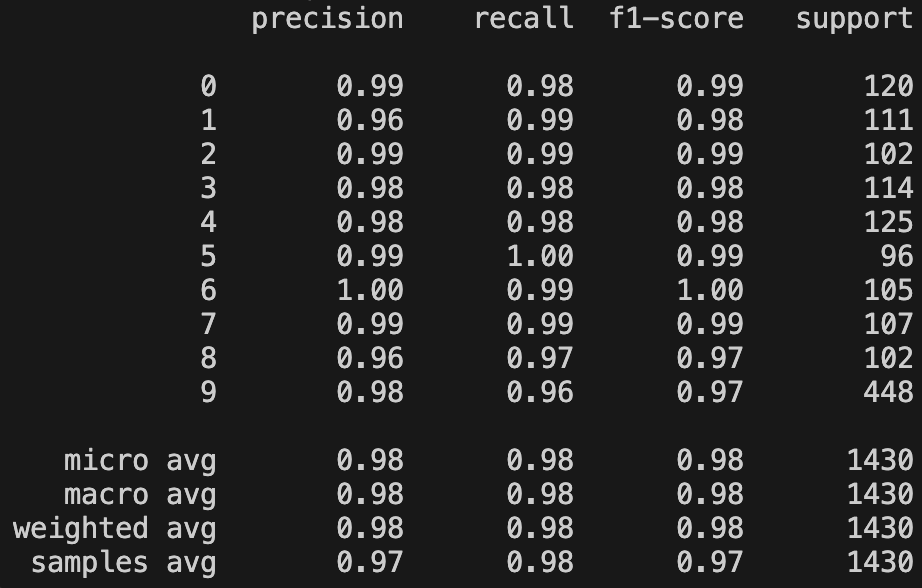
\includegraphics[width=0.7\textwidth]{Report_MLP.png}
    \caption{ معیارهای ارزیابی برای تشخیص علائم دست در مدل شبکه چند لایه‌ای پرسپترونی}
\end{figure}

\begin{figure}[h]
    \centering
    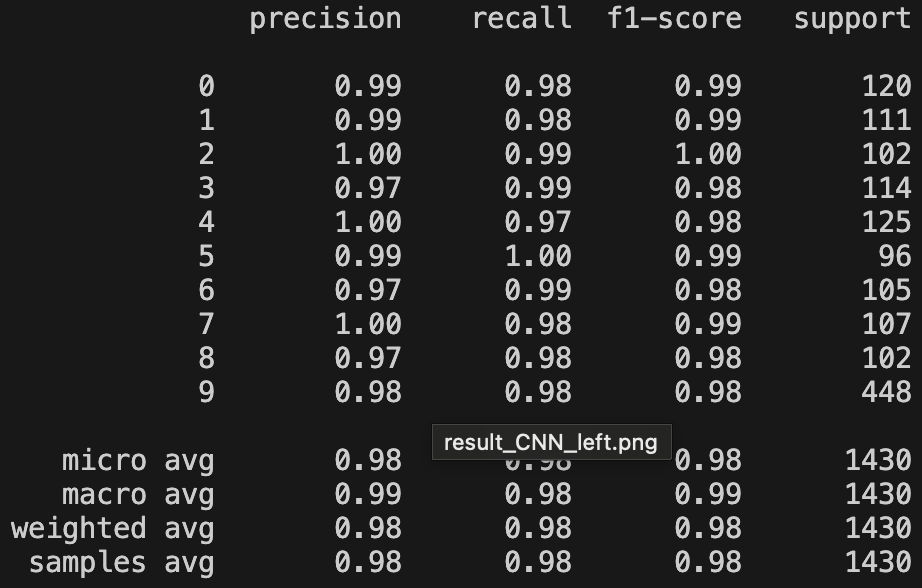
\includegraphics[width=0.7\textwidth]{Report_CNN.png}
    \caption{ معیارهای ارزیابی برای تشخیص علائم دست در مدل شبکه عصبی پیچشی}
\end{figure}

\begin{figure}[h]
    \centering
    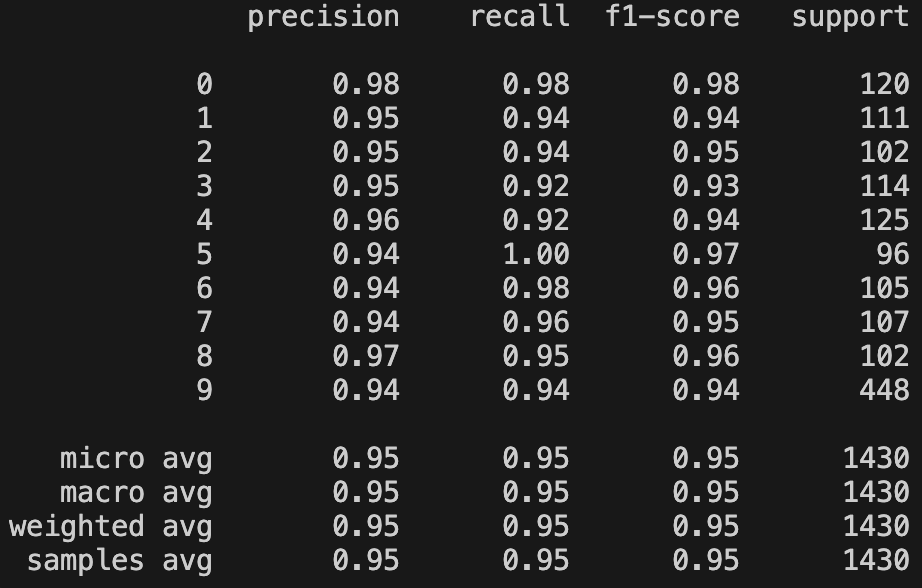
\includegraphics[width=0.7\textwidth]{Report_LSTM.png}
    \caption{ معیارهای ارزیابی برای تشخیص علائم دست در مدل شبکه حافظه طولاني كوتاه مدت}
\end{figure}

\begin{figure}[h]
    \centering
    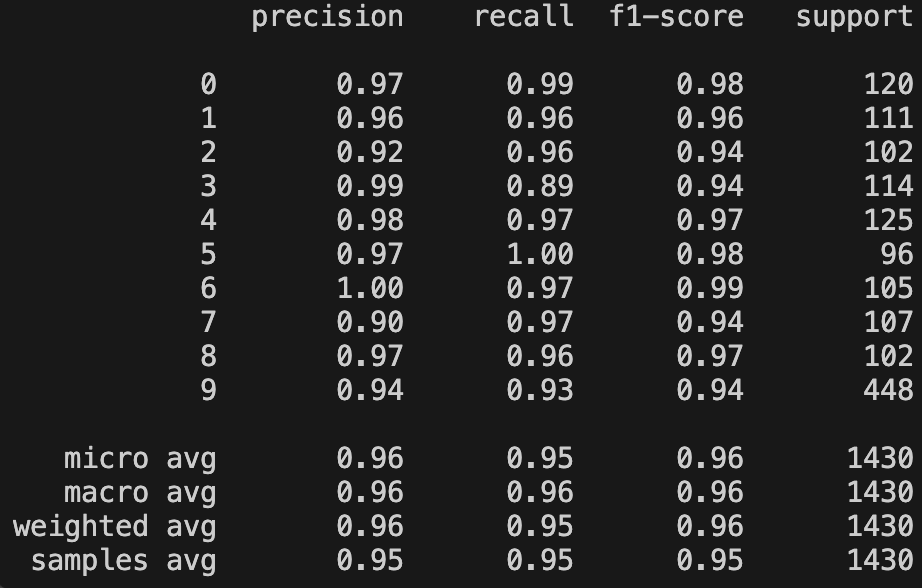
\includegraphics[width=0.7\textwidth]{Report_RNN.png}
    \caption{ معیارهای ارزیابی برای تشخیص علائم دست در مدل شبکه عصبي بازگشتي}
\end{figure}

\subsection[ماتریس درهم‌ریختگی]{ماتریس درهم‌ریختگی\protect\LTRfootnote{Confusion Matrix}}
ماتریس درهم‌ریختگی یک ابزار مهم در ارزیابی عملکرد مدل‌های طبقه‌بندی است. این ماتریس نشان‌دهنده تعداد نمونه‌هایی است که به درستی به هر کلاس تخصیص یافته‌اند و همچنین تعداد نمونه‌هایی که به اشتباه به کلاس‌های دیگر تخصیص داده شده‌اند. به عبارت دیگر، هر سطر این ماتریس نشان‌دهنده کلاس واقعی است و هر ستون نشان‌دهنده کلاسی است که مدل پیش‌بینی کرده است. اگر خانه \lr{ij} این ماتریس، عدد \lr{n} را داشته باشد، این به این معنا است که مدل \lr{n} بار نمونه‌های کلاس \lr{i} را به درستی به کلاس \lr{j} تخصیص داده است.
\\
ماتریس درهم‌ریختگی حاوی اطلاعات مفیدی است زیرا به ما اطلاعات دقیقی از عملکرد مدل در هر کلاس را می‌دهد. از این اطلاعات می‌توان برای ارزیابی عملکرد کلی مدل، شناسایی نقاط ضعف و قوت مدل، و بهبود آن استفاده کرد. همچنین، این ماتریس به ما امکان می‌دهد بررسی کنیم که آیا مدل ما به نسبت هر کلاس اشتباه می‌کند یا اشتباهات آن به کلاس‌های خاصی متمرکز شده‌اند \cite{Confusio72:online}.

\begin{figure}[h]
    \centering
    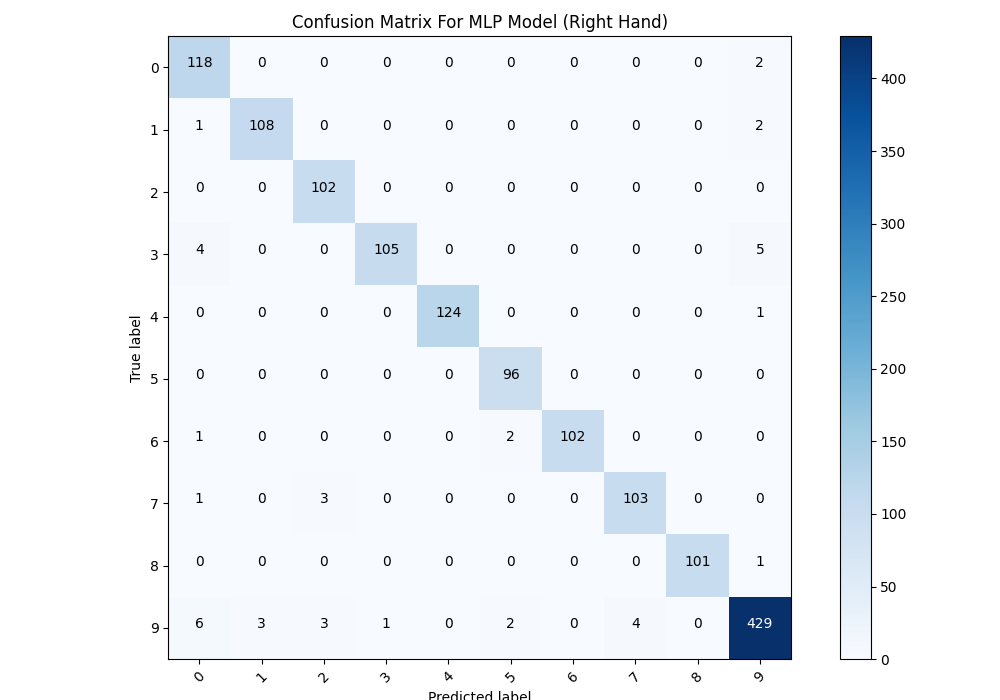
\includegraphics[width=0.8\textwidth]{Matrix_MLP_right.png}
    \caption{ماتریس درهم‌ریختگی در مدل شبکه عصبی چندلایه‌ای پرسپترونی}
\end{figure}


\begin{figure}[h]
    \centering
    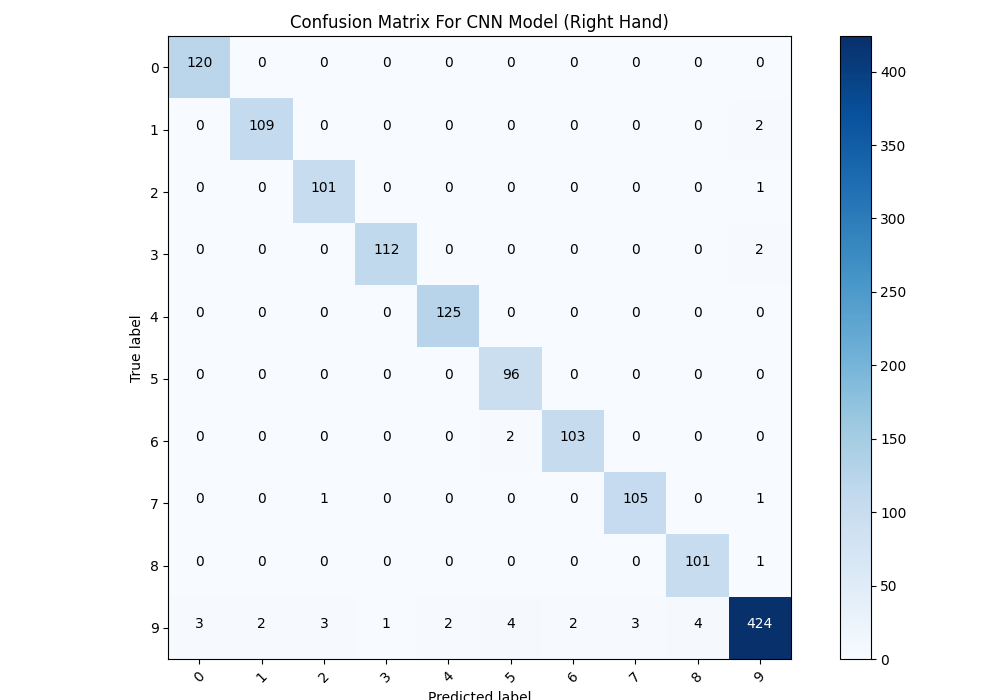
\includegraphics[width=0.8\textwidth]{Matrix_CNN_right.png}
    \caption{ ماتریس درهم‌ریختگی در مدل شبکه عصبی پیچشی}
\end{figure}


\begin{figure}[h]
    \centering
    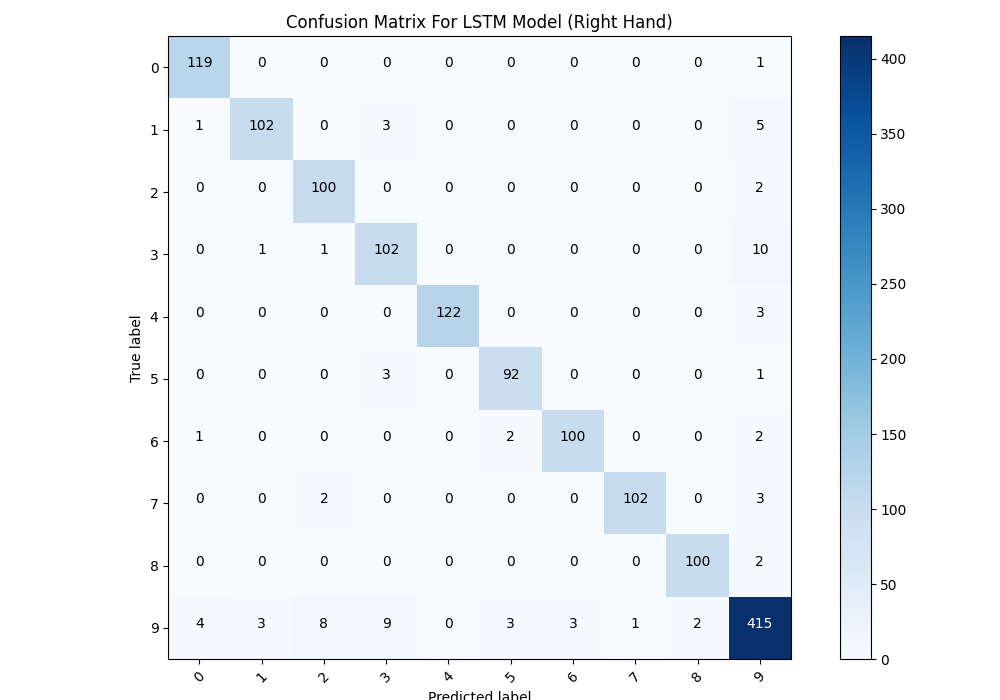
\includegraphics[width=0.8\textwidth]{Matrix_LSTM_right.png}
    \caption{ ماتریس درهم‌ریختگی در مدل شبكه حافظه طولاني كوتاه مدت}
\end{figure}


\begin{figure}[h]
    \centering
    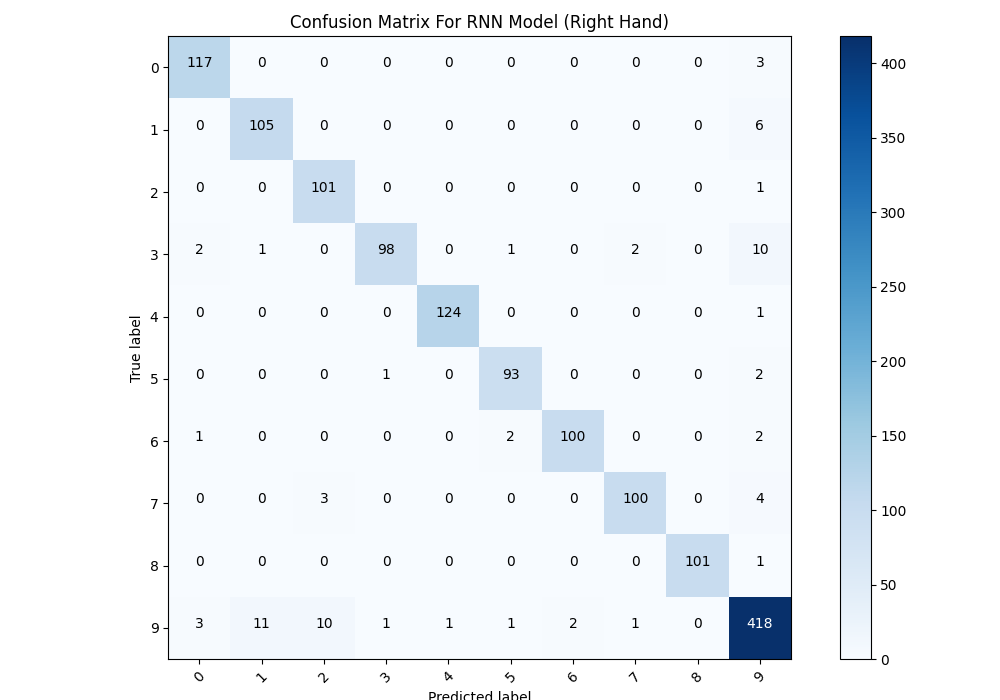
\includegraphics[width=0.8\textwidth]{matrix_RNN_right.png}
    \caption{ ماتریس درهم‌ریختگی در مدل شبکه عصبي بازگشتي}
\end{figure}


\section[نمودار‌های دقت و خطا بر حسب دوره]{ نمودار‌های دقت و خطا بر حسب دوره \LTRfootnote{Epoch}}
یک دوره زمانی است که کل مجموعه داده تنها یک بار از طریق شبکه عصبی انتشار پیدا کرده و پس از آن پس انتشار اتفاق میافتد
. از آنجایی که یک دوره ممکن است بسیار بزرگ باشد و نتوان آن را به یکباره به سیستم وارد کرد، به چند دسته کوچکتر تحت عنوان "دسته\LTRfootnote{Batch}" تقسیم می‌شود. انتقال کل مجموعه داده از طریق یک شبکه عصبی به تنهایی کافی نیست و باید مجموعه داده را چندین بار به شبکه ارسال کرد. در این پروژه، از یک مجموعه داده محدود استفاده شده و برای بهینه‌سازی یادگیری آن از الگوریتم گرادیان نزولی استفاده می‌کنیم.
\\
تعیین تعداد صحیح دوره‌ها از اهمیت بالایی برخوردار است. با افزایش تعداد دوره‌ها،‌ تعداد دفعات تغییر وزن در شبکه عصبی بیشتر می‌شود و منحنی یادگیری از حالت کم‌برازش\LTRfootnote{Underfitting} به حالت بهینه\LTRfootnote{Optimal} و در نهایت به حالت بیش‌برازش\LTRfootnote{Overfitting} تغییر می‌یابد. تعداد دوره‌ها باید به گونه‌ای تعیین شود که تعادلی برقرار شود و بتوان منحنی یادگیری را به بهترین حالت ممکن رساند.
\\
در این پروژه، به منظور نظارت و ارزیابی عملکرد مدل، نمودارهای دقت و خطا بر حسب دوره ترسیم شده‌اند. این نمودارها نشان می‌دهند که چگونه دقت مدل و میزان خطا در طول زمان تغییر می‌کنند. بررسی این نمودارها می‌تواند به شناسایی نقاط بهینه و جلوگیری از بیش‌برازش کمک کند.


\begin{figure}[h]
    \centering
    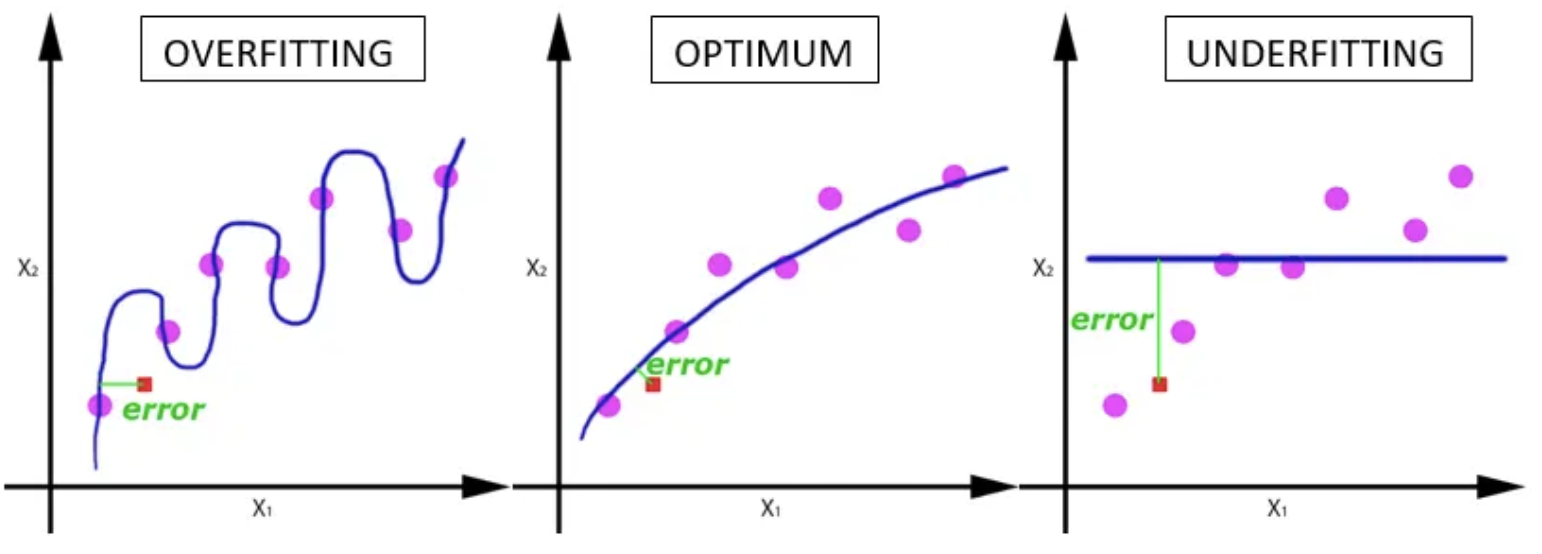
\includegraphics[width=1\textwidth]{fitting.png}
    \caption[منحنی‌ حالت‌های کم‌برازش، بهینه و بیش‌برازش]{منحنی‌ حالت‌های کم‌برازش، بهینه و بیش‌برازش \cite{wwwreddi92:online}}
\end{figure}

\begin{figure}[h]
    \centering
    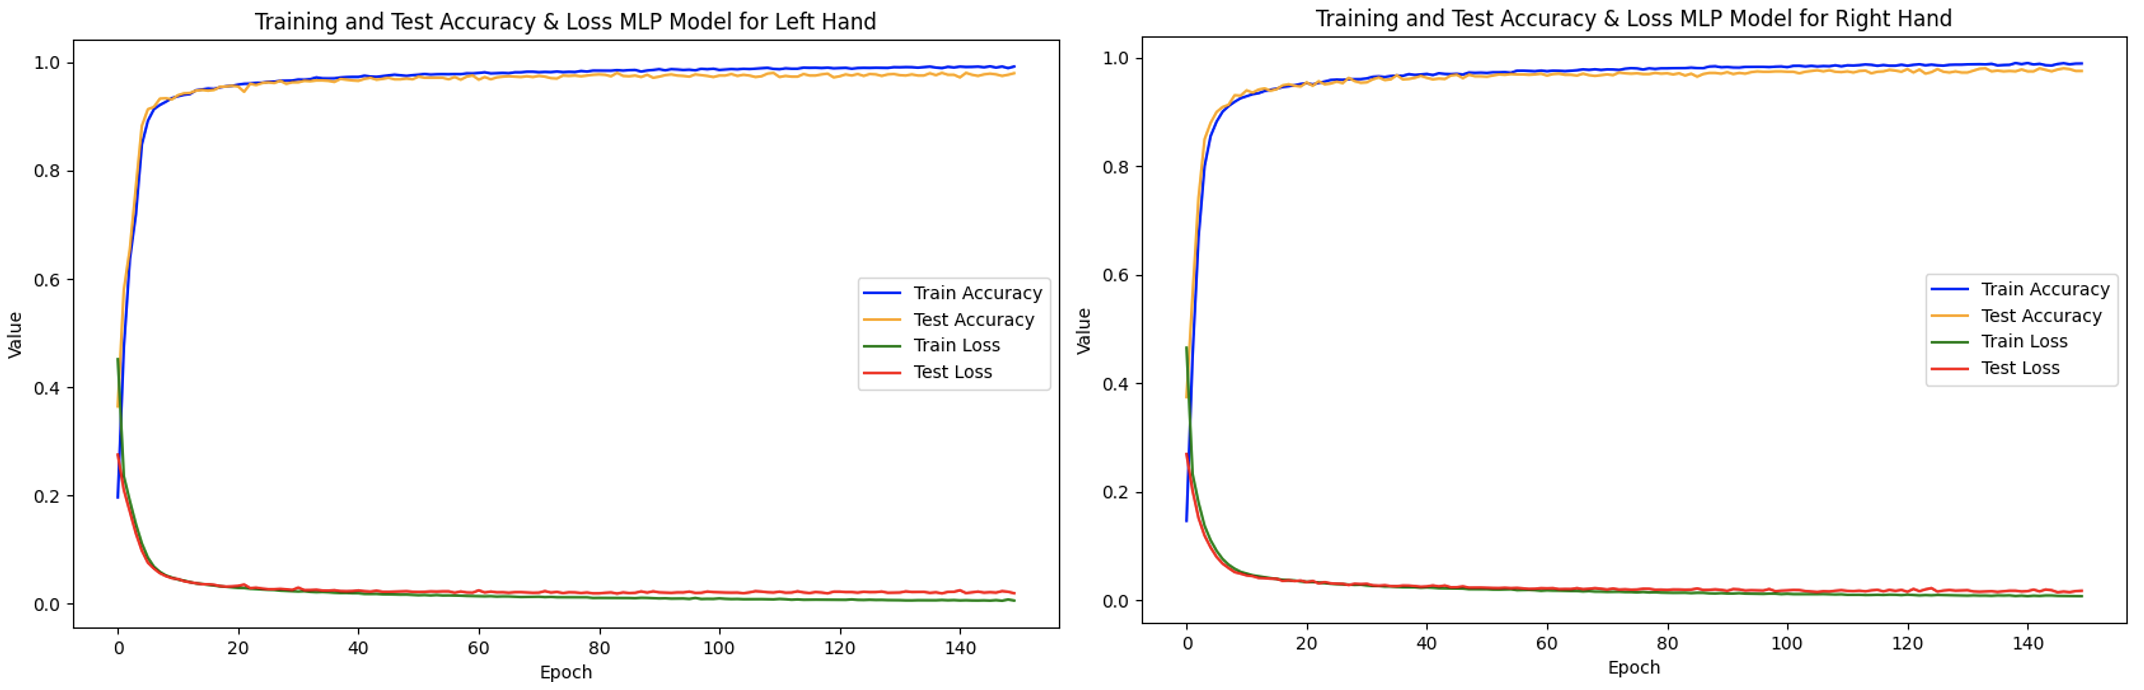
\includegraphics[width=1\textwidth]{Chart_MLP.png}
    \caption{نمودار روند دقت و خطا در دست‌های راست و چپ بر حسب دوره در داده‌های آموزش و تست در مدل شبكه عصبي چندلايه پرسپتروني}
\end{figure}

\begin{figure}[h]
    \centering
    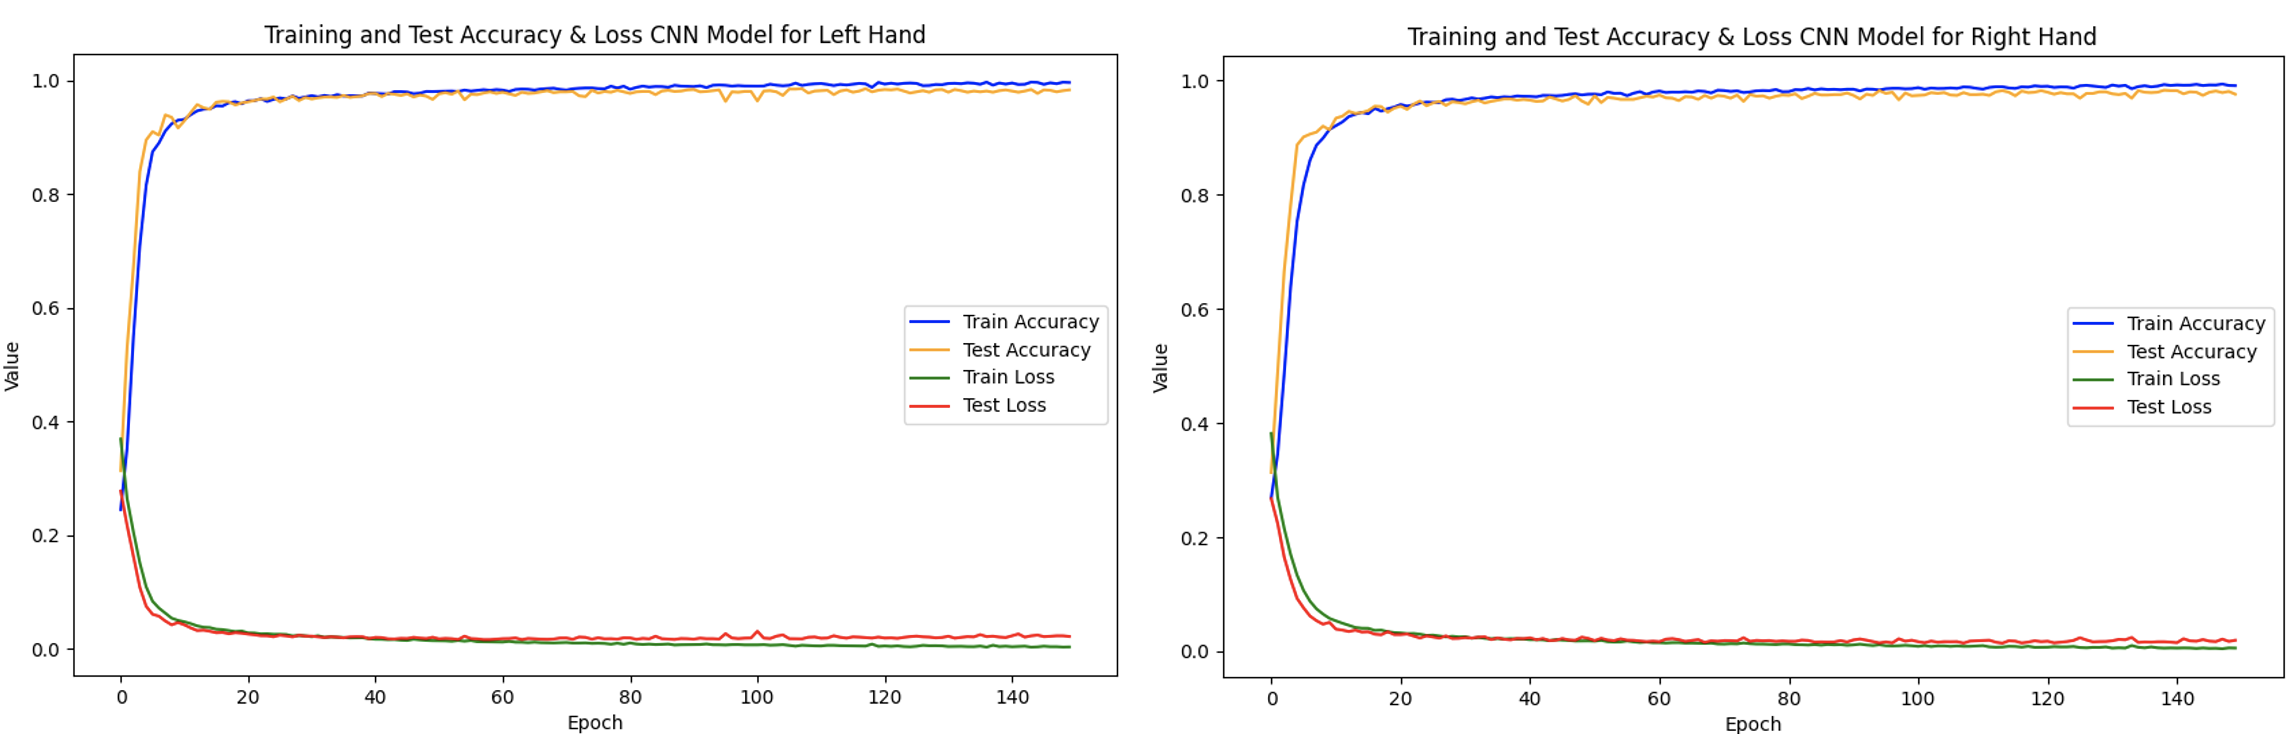
\includegraphics[width=1\textwidth]{Chart_CNN.png}
    \caption{نمودار روند دقت و خطا در دست‌های راست و چپ بر حسب دوره در داده‌های آموزش و تست در مدل شبکه عصبی پیچشی}
\end{figure}

\begin{figure}[h]
    \centering
    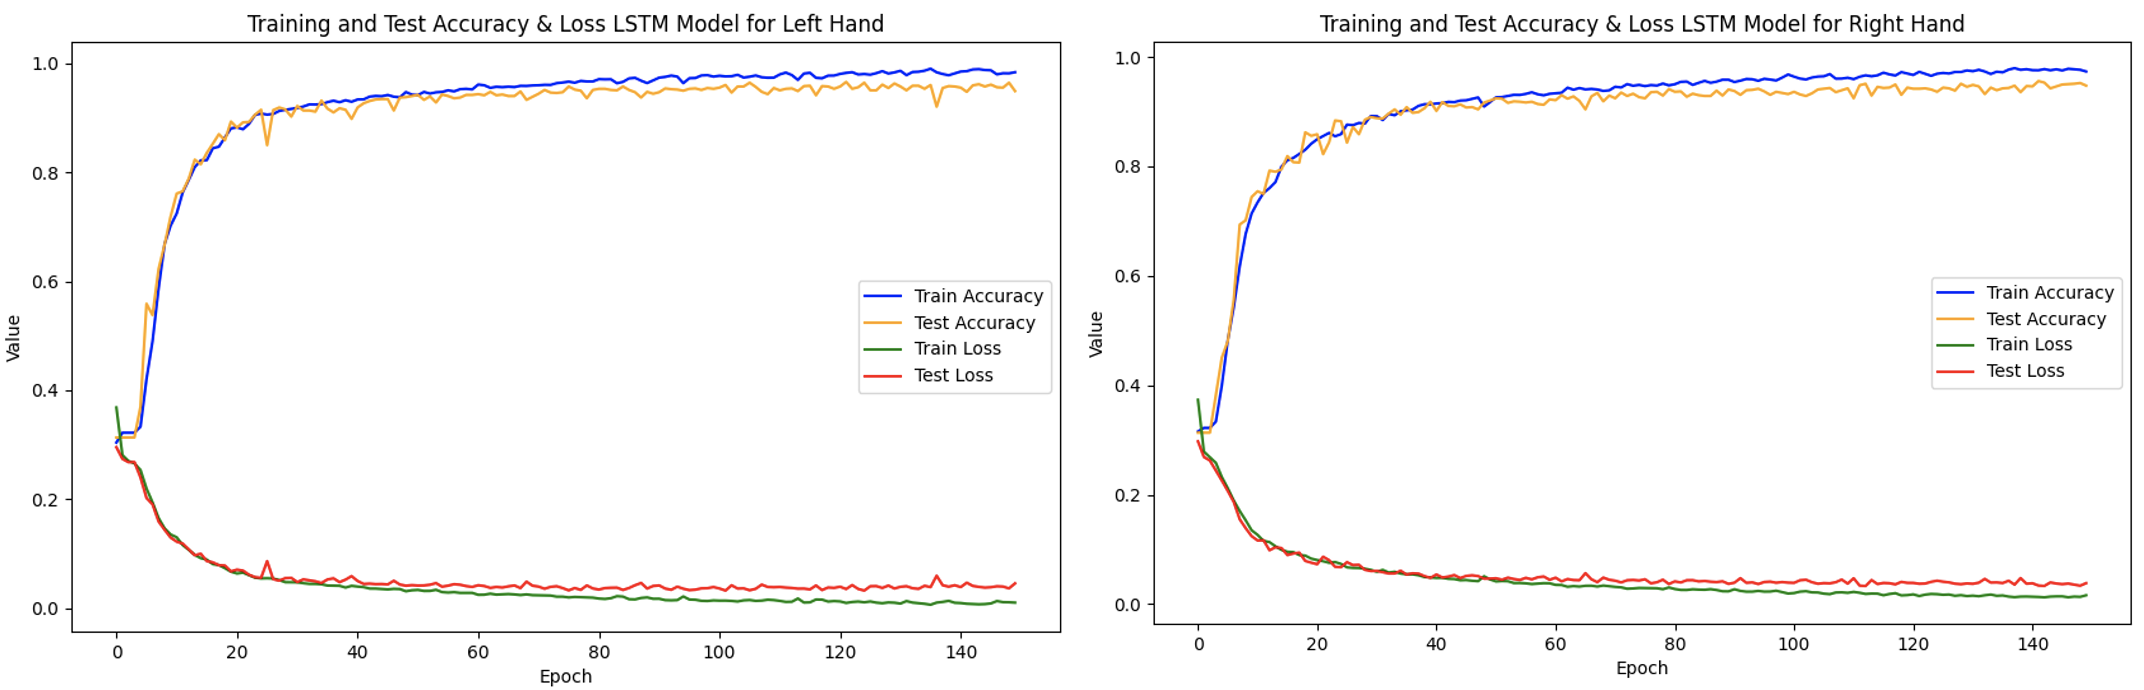
\includegraphics[width=1\textwidth]{Chart_LSTM.png}
    \caption{نمودار روند دقت و خطا در دست‌های راست و چپ بر حسب دوره در داده‌های آموزش و تست در مدل شبكه حافظه طولاني كوتاه مدت}
\end{figure}

\begin{figure}[h]
    \centering
    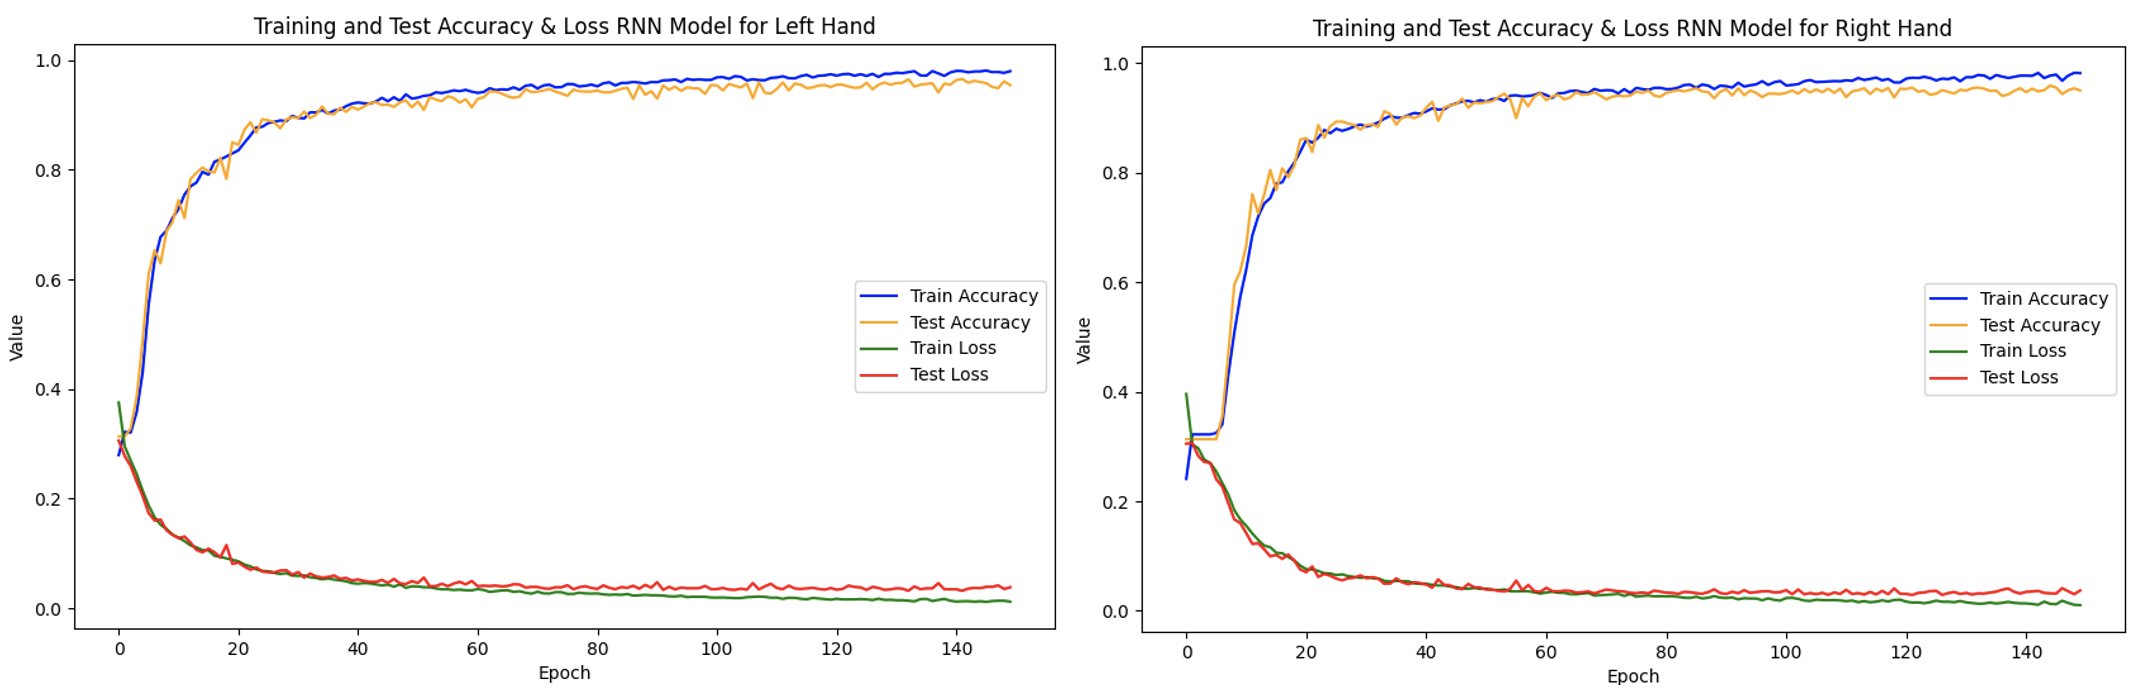
\includegraphics[width=1\textwidth]{Chart_RNN.png}
    \caption{نمودار روند دقت و خطا در دست‌های راست و چپ بر حسب دوره در داده‌های آموزش و تست در مدل شبكه عصبي بازگشتي}
\end{figure}


\section{تاثیر پس‌پردازش رأی‌گیری پنجره‌ای بر دقت}
به طور کلی با توجه به 
\cref{table:window}
 دقت ما پس از پیاده‌سازی رأی‌گیری پنجره‌ای کاهش پیدا کرده است. اما لزوم این الگوریتم برای ما از اهمیت ویژه‌ای برخوردار است, چرا که در بیشتر مواردی که دقت به درستی بیان نشده است در زمانی است که علائم دست کاربر نمادی را نشان داده اما پهپاد از آن پیروی نمی‌کند. این موضوع می‌تواند سبب ناخوشایندی کاربر شود، اما این الگوریتم سبب شده است تا بسیاری از
 مواردی که علائم دست در یک یا تعداد کمی از فریم‌ها توسط سیستم اشتباه برداشت شده‌است، یا حتی کاربر در مدت کوتاهی به اشتباه هدف خود را بیان کند، دستور نهایی صادر نشود تا پهپاد دچار مشکل نشود.

\begin{table}[h!]
    \centering
    \begin{tabular}{||>{\centering\arraybackslash}p{5.5cm} >{\centering\arraybackslash}p{4cm} >{\centering\arraybackslash}p{4cm}||}
     \hline
     \rule{0pt}{3ex} معماری مدل & دقت مدل بدون رأی‌گیری پنجره‌ای & دقت مدل با رأی‌گیری پنجره‌ای \\ [1.5ex]
     \hline
     \hline
     \rule{0pt}{0.5ex} & & \\  
     شبکه عصبی چندلایه‌ای پرسپترونی & 6 & 7 \\ [2.5ex]
     شبکه عصبی پیچشی & 7 & 8 \\ [2.5ex]
     شبکه عصبی حافطه طولانی کوتاه مدت & 5 & 8 \\ [2.5ex]
     \hline
    \end{tabular}
    \caption{جدول ارزیابی تاثیر دقت در رأی‌گیری پنجره‌ای}
    \centering
    \label{table:window}
\end{table}


\section{سرعت اجرای برنامه}
به منظور رسیدن به یکی از اهداف اصلی این پروژه، که بی‌درنگ بودن آن می‌باشد، لازم است که میزان پاسخ‌گویی مدل‌ها نیز مورد بررسی و ارزیابی قرار گیرد. در 
\cref{table:1}
زمان پاسخ‌گویی مدل‌ها از زمانی که داده‌ها از طریق دوربین خوانده می‌شوند تا زمانی که دستور به پهپاد داده می‌شود، آورده شده است.

\begin{table}[h!]
    \centering
    \begin{tabular}{||c c||}
     \hline
     \rule{0pt}{3ex}معماری مدل & زمان پاسخگویی مدل\\ [1.5ex]
     \hline
     \hline
     \rule{0pt}{0.5ex} & \\  % Adds space before the first data row, while keeping the vertical lines
     شبکه چندلایه‌ای پرسپترونی & 4 $\pm$ 39 میلی‌ثانیه \\ [2.5ex]
     شبکه عصبی پیچشی & 7 $\pm$ 41 میلی‌ثانیه  \\ [2.5ex]
     شبکه عصبی  حافظه طولانی کوتاه مدت & 1 $\pm$ 44 میلی‌ثانیه  \\ [2.5ex]
     شبكه عصبي بازگشتي & 2 $\pm$ 41 میلی‌ثانیه  \\ [2.5ex]

     \hline
    \end{tabular}
    \caption{جدول ارزیابی زمان پاسخگویی مدل‌ها}
    \label{table:1}
\end{table}

% شبکه چندلایه‌ای پرسپترونی & 4.0 $\pm$ 9.3 میلی‌ثانیه \\ [2.5ex]
%  شبکه عصبی پیچشی & 7.0 $\pm$ 1.4 میلی‌ثانیه  \\ [2.5ex]
%  شبکه عصبی  حافظه طولانی کوتاه مدت & 1 $\pm$ 4.4 میلی‌ثانیه  \\ [2.5ex]
%  شبكه عصبي بازگشتي & 9.0 $\pm$ 1.4 میلی‌ثانیه  \\ [2.5ex]


\section{سخت‌افزار مورد نیاز}
این پروژه باید به گونه‌ای اجرا می‌شد که بر روی ساده‌ترین سیستم‌های کامپیوتری نیز قابل اجرا باشد، زیرا سخت‌افزار پهپادها به‌طور معمول دارای پردازنده‌های ضعیف‌تری هستند. همچنین، استفاده از پردازنده گرافیکی ممکن نبود، چرا که پهپادها فاقد پردازنده‌های گرافیکی می‌باشند. 
معماری‌های پیاده‌سازی شده به نحوی طراحی شدند که تعادل میان دقت و بهره‌وری از سخت‌افزار حفظ شود، به طوری که هم قابلیت اجرا به صورت بی‌درنگ را داشته باشند و هم امکان پیاده‌سازی آن‌ها بر روی پهپاد فراهم باشد. از این رو، معماری‌ها به گونه‌ای پیاده‌سازی شدند که بر روی پردازنده اجرا شوند.
میزان استفاده از پردازنده برای اجرای معماری‌های پیاده‌سازی شده در این پروژه به شرح زیر است:



\begin{table}[h!]
    \centering
    \begin{tabular}{||c c c||}
     \hline
     \rule{0pt}{3ex}معماری مدل & پردازنده & فضای ذخیره‌شده \\ [1.5ex]
     \hline
     \hline
     \rule{0pt}{0.5ex} & & \\  % Adds space before the first data row, while keeping the vertical lines
     شبکه چندلایه‌ای پرسپترونی & 6 & 6 \\ [2.5ex]
     شبکه عصبی پیچشی & 7 & 6 \\ [2.5ex]
     شبکه عصبی  حافظه طولانی کوتاه مدت & 5 & 6 \\ [2.5ex]
     \hline
    \end{tabular}
    \caption{جدول ارزیابی سخت‌افزار موردنیاز مدل‌ها}
    \label{table:4}
\end{table}

\section{مقایسه دقت پروژه با کارهای مشابه}
پروژه پیاده‌سازی از دقت بسیار بالایی برخوردار است که این دقت به دلیل ترکیب پیش‌پردازش، کتابخانه مدیاپایپ، مدل کلاس‌بندی و پس‌پردازش است. 
\\ در این قسمت به مقایسه دقت پروژه پیاده‌سازی شده با پروژه‌های مشابه با هدف کنترل پهپاد با کمک تشخیص علائم دست پرداخته‌ایم.

\begin{table}[h!]
    \centering
    \begin{tabular}{||>{\centering\arraybackslash}p{10.5cm} >{\centering\arraybackslash}p{2cm} >{\centering\arraybackslash}p{2cm}||}
     \hline
     \rule{0pt}{3ex} نام مقاله & تعداد علائم‌های دست & دقت تشخیص علائم دست \\ [1.5ex]
     \hline
     \rule{0pt}{0.5ex} & & \\  
     برنامه ما & 9 & 6 \\ [2.5ex]
     پهپادهاي كنترل شده با علائم دست به صورت متن باز\cite{natarajan2018hand} & 5 & ۴۷۱.۹۷ \\ [2.5ex]
     روشهاي تشخيص علائم دست به صورت بي‌درنگ\cite{fang2007real} & 6 & 8.93 \\ [2.5ex]
     تشخيص علائم دست براي كنترل پهپاد با استفاده از ياديگيري عميق\cite{hadri2018hand} & 9 & 3.83  \\ [2.5ex]
     علائم يوايوي: مجموع‌داده براي يوايوي كنترل و تشخيص علائم\cite{perera2018uav} & 13 & 9.91 \\ [2.5ex]
     تشخيص علائم دست براي استفاده‌هاي بي‌درنگ\cite{murugeswari2014hand} & 6 & 8.90 \\ [2.5ex]
     روشي بهبود يافته براي تشخيص علائم دست با استفاده از نقاط كليدي و جعبه مرزي\cite{dang2022improved} & 6 & 94 \\ [2.5ex]
     تشخیص حرکت دست با استفاده از تکنیک های بینایی ماشین\cite{rios2013hand} & 6 & 1.93 \\ [2.5ex]
     تشخیص علائم دست با استفاده از تکنیک‌های پردازش تصویر و استخراج ویژگی\cite{sharma2020hand} & 28 & 54.89 \\ [2.5ex]
     استفاده از تشخیص حرکت دست برای برنامه راهنمای کاربر با استفاده از مدیاپایپ\cite{harris2021applying} & 10 & 95 \\ [2.5ex]
     دست‌هاي مدياپايپ: تشخيص بي درنگ دست بر روي دستگاه‌ها\cite{zhang2020mediapipe} & 8 & 7.94 \\ [2.5ex]
     سیستم تشخیص حرکت دست مبتنی بر بینایی کامپیوتر و یادگیری ماشین\cite{trigueiros2015hand} & 28 & 72.93 \\ [2.5ex]
     تشخیص علائم دست با استفاده از مدل های پنهان مارکوف\cite{min1997hand} & 5 & 1.92 \\ [2.5ex]
     تشخیص علائم دست با استفاده از کینکت\cite{li2012hand} & 38 & 84 \\ [2.5ex]
     تشخیص علائم دست با استفاده از شبکه های عصبی\cite{murthy2010hand} & 10 & 89 \\ [2.5ex]
     \hline
    \end{tabular}
    \caption{جدول مقایسه پروژه با کارهای مشابه}
\end{table}

\pagebreak


\section{جمع‌بندی}
مدل‌های ارائه شده در این پروژه دارای دقت و کارایی مناسبی هستند که امکان استفاده آن‌ها در کاربردهای واقعی را فراهم می‌کند. این مدل‌ها قادرند به خوبی علائم‌های دست را تشخیص داده و از آن‌ها در عملیات مختلفی مانند کنترل دستگاه‌ها و رابط‌های کاربری استفاده شوند.
\\
علاوه بر این، با مقایسه عملکرد  این پروژه با کارهای مشابه در حوزه تشخیص علائم‌های دست، مشخص شده است که پروژه ما دارای دقت مشابه یا حتی بالاتری است، به ویژه اگر تعداد کلاس‌های علائم دست در نظر گرفته شود. این نکته نشان می‌دهد که مدل‌های ارائه شده به خوبی تنوع و پیچیدگی علائم‌های دست را درک می‌کنند و قادر به تشخیص آن‌ها هستند، که این امر یکی از چالش‌های اصلی در این زمینه است.
\\
با توجه به این نتایج، می‌توانیم اطمینان داشته باشیم که پروژه ما قادر است به عنوان یک راه‌حل کارآمد برای تشخیص علائم‌های دست در برنامه‌ها و سیستم‌های واقعی مورد استفاده قرار بگیرد.
در فصل بعدی به یک جمع‌بندی کلی این پروژه و ارائه پیشنهاداتی برای بهبود عملکرد سیستم طراحی شده می‌پردازیم.

